\section{Methodology}
In our project we have built an end-to-end speech recognition system. The system has been trained on some specific speech commands and it can recognize those commands with a certain amount of accuracy. The general architecture of the system is given in figure \ref{fig1}.
\begin{figure}[!htb]
\centerline{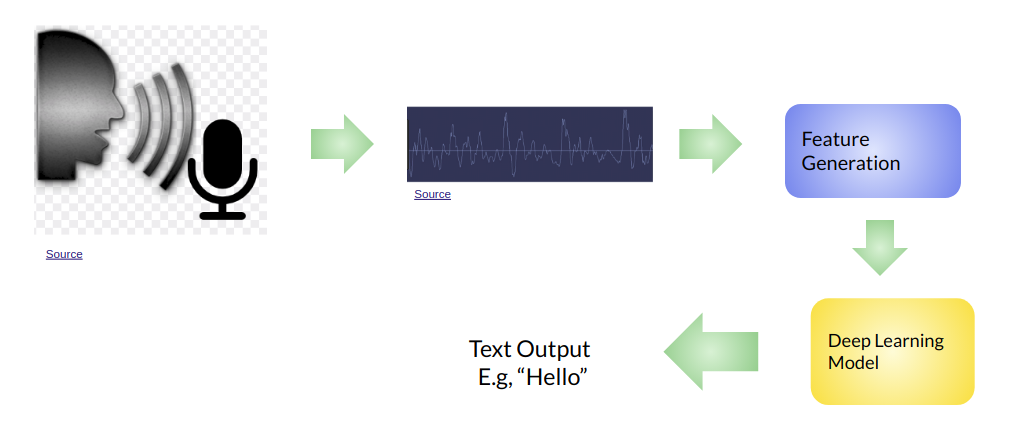
\includegraphics[height=60mm,width=95mm]{img/fig1.png}}
\caption{General architecture of the speech recognition system}
\label{fig1}
\end{figure}
\par First, data has been collected by recording specific words at a certain sample rate and of length of 1 second. This speech data has been converted to samples where each sample represent the amplitude of the sound on that specific instant of time. After this, relevant features has been extracted out of that sampled speech data e.g, mel-frequency cepstral co-efficient (MFCC), spectrogram etc. These features will be feeded to our model for training. After training, we have tested on some test speech data which has been processed by the model and produced text output of that test data. 
\par In this section we will first discuss the background theory behind the speech recognition system. Then, we will discuss about our best model's architecture and also about the other approach.


\subsection{Background Theory}
In our project we have used spectrogram as our primary feature. Thus first we have used convolutional neural networks (CNN) for extracting the relevant information from spectrogram images. Then this relevant information about the image has been flattened and provided as input to the next gated recurrent unit (GRU) layer. Hence, we will give a brief introduction about CNN and GRU. 

\subsubsection{Convolutional Neural Network (CNN)}
CNN presumes that the input will be an image certain height, width and depth. The general architecture of CNN is given in figure \ref{fig2}. There are two kinds of layers present in CNN. They are described below: 
\begin{itemize}
    \item \textbf{Convolution Layer: }In this layer we perform convolution operation on the input image using some filter. The operation is then slided to to next block of pixels in the image and the result of this operation will be a scaled down 2D feature matrix which will be provided as input to the pooling layer. 
    \item \textbf{Pooling Layer: }We insert pooling layers in between two convolution layers.``Its function is to progressively reduce the spatial size of the representation to reduce the amount of parameters and computation in the network, and hence to also control over-fitting"\cite{b1}. In pooling layers we also use the filters but perform a MAX operation, i.e, maximum value in a window of pixel is chosen.
\end{itemize}
\begin{figure}[!htb]
\centerline{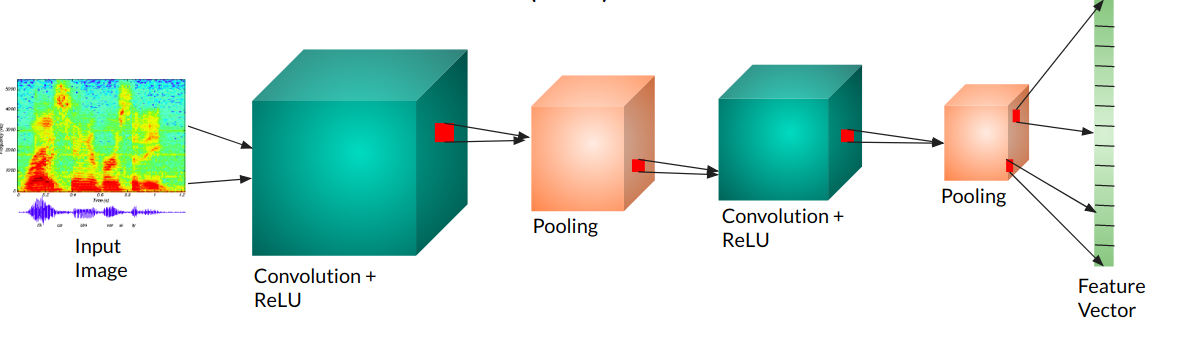
\includegraphics[height=40mm,width=95mm]{img/fig2.png}}
\caption{General architecture of CNN}
\label{fig2}
\end{figure}

\subsubsection{Gated Recurrent Unit (GRU)}
GRU is a special case of recurrent neural network (RNN). GRU solves the vanishing gradient problem of RNN. In GRU, two new concept of gates has been introduced to eliminate the problem of vanishing gradient. These gates generally decide what output information will be provided to the next stage. They are described below : 
\begin{itemize}
    \item \textbf{Update Gate: } In this gate we calculate the output of one computation unit using the formula $$z_t=\sigma(W^{(z)}x_t+U^{(z)}h_{t-1})$$
    $x_t$ is the input to the computation unit at time instant $t$ and $W^{z}$ is its weight vector. $h_{t-1}$ holds the past information of the previous computation unit and $U^{(z)}$ holds the weight of previous $t-1$ units. $\sigma$ is the sigmoid function which we apply to the whole expression to scale down the value between 0 to 1. Update gate decides about the amount of information that has to be passed to the future computation units.
    \item \textbf{Reset Gate: }``It is used to decide about the amount of information from the past that is needed to forget" \cite{b2}. The formula for this is $$r_t=\sigma(W^{(r)}x_t+U^{(r)}h_{t-1})$$
\end{itemize}
The general architecture of a GRU is given in figure \ref{fig3}.
\begin{figure}[!htb]
\centerline{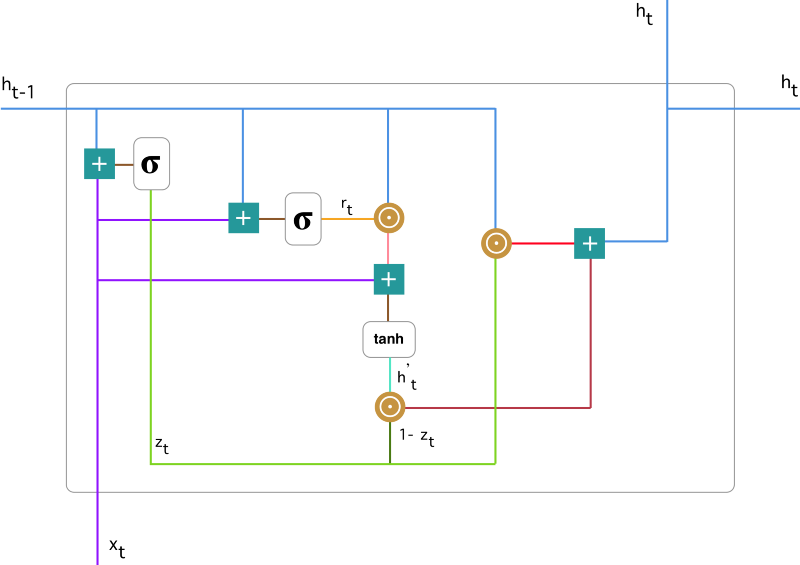
\includegraphics[height=60mm,width=90mm]{img/fig3.png}}
\caption{General architecture of GRU \cite{b2}}
\label{fig3}
\end{figure}

\subsection{Model Architecture}
We have implemented our model with \textit{Keras} library \cite{b3} in \textit{Python 3.6}. The arhitecture of the model is given in figure \ref{fig4}. 
\begin{figure*}
\centerline{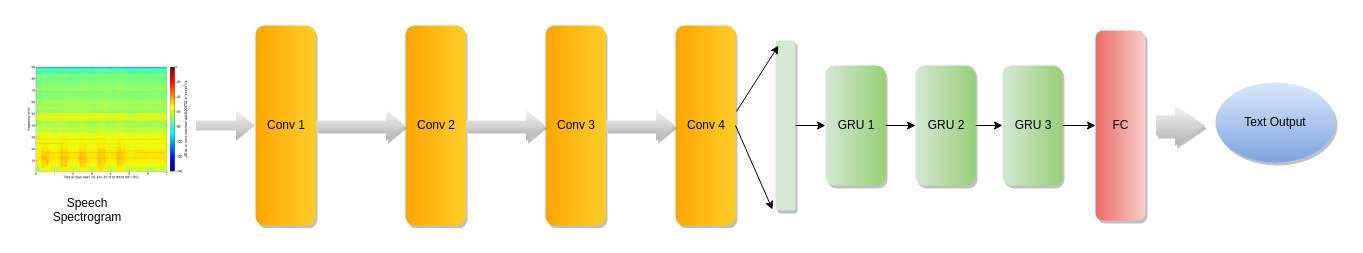
\includegraphics[height=50mm,width=200mm]{img/fig4.png}}
\caption{Architecture of the model}
\label{fig4}
\end{figure*}
Spectrogram of the audio data has been given as input to our model. As spectrogram is a visual interpretation of the audio data thus we have passed the spectrogram through four layers of CNN and then through three layers of GRU. 
CNN will extract all the relevant features in each layer and at the fourth layer it is fetching the most prominent features from the spectrogram.
\par Features collected from convolutional layers will be flattened and then feeded to as the audio is a sequence of phonemes thus we have passed the features extracted from CNN to GRU layers. It will extract the sequencing features of phonemes that are present in the audio data. 
\par Finally, the fully connected layers with softmax function is used to at the end to get all the probabilities of 10 classes. We have used cross-entropy as loss function along with Adam optimizer for back-propagation. Also the learning rate was 0.001 and dropouts has been used with the rate of 30\%. The number of iteration were 50 for optimization. 


\subsection{Other Approach}
We have tried another model with only CNN layers. We had introduced four convolutional layers followed by max pooling layers. And as input to the CNN we had used mel-frequency cepstral co-efficients (MFCC). But CNN did not worked with this feature of audio. And as we were increasing the number of layers after the fourth layer, the test accuracy was decreasing continuously.